\documentclass[headsepline=true, footsepline=true]{scrartcl}

\usepackage{tutorial}

% % ==============================================================
\title{Separates Deployment von Produktdaten}
\author{Cornelius Dirmeier}
\setcopyright{
\includegraphics[height=10pt]{./pics/FaktorZehn-ORG.png}}
% % ==============================================================

\begin{document}

\maketitle

\section{Einleitung}

Faktor-IPS verwaltet Produktdaten während der Produktentwicklung in XML Dateien.
Zur Laufzeit wurde bis Version 2.5 ausschließlich mit XML
Dateien gearbeitet. Genau genommen muss man von XML-Ressourcen sprechen, da die
einzelnen XML-Dateien meist in Bibliotheken (z.B. JAR-Dateien) zusammengefasst
werden. Um die Produktdaten zu laden müssen sie zur Laufzeit im Classpath der
Applikation verfügbar sein, entweder als einzelne Dateien oder in Form von
Bibliotheken. Innerhalb einer Applikation kann auf die Produktdaten über ein
Runtime Repository (z.B. $ClassloaderRuntimeRepository$) zugegriffen werden.

\begin{figure}[htb] \centering
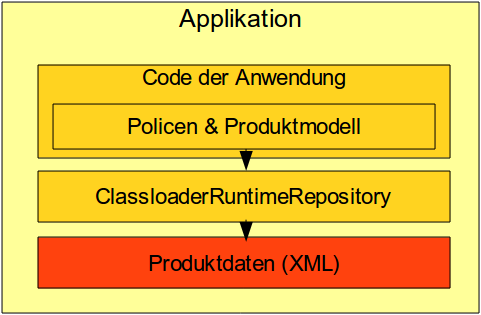
\includegraphics[width=8cm]{./pics/old_architecture.png} \caption{Bisher wurden
Programmcode und Produktdaten in einer gemeinsamen Applikation ausgeliefert}
\label{old_architecture}
\end{figure}

Da sowohl Programmcode als auch Produktdaten als Dateien vorliegen, können sie
zusammen in einem Werkzeug wie CVS oder Subversion gespeichert werden. Eine
fertige Version von Programmcode und Produktdaten wird dann in eine Zielumgebung
transportiert. Im JavaEE Umfeld wird dazu ein Enterprise Archive (EAR) bzw. ein
Web Application Archive (WAR) erzeugt.

Werden die Produktdaten verändert oder erweitert muss dieses Archiv ausgetauscht
werden. Da Produktdaten und Programmcode eine Einheit bilden, muss auch der
Programmcode neu ausgeliefert werden.

Ziel des separaten Deployments von Produktdaten ist es, bei einer Änderung der
Produktdaten nur die XML-Ressourcen auszutauschen ohne den Programmcode neu
ausliefern zu müssen. Die dabei auftretenden Herausforderungen und die daraus
entwickelten Lösungen werden in diesem Dokument vorgestellt.

\section{Herausforderungen}

\subsection{Runtime Repository}

Für den Zugriff auf die Produktdaten steht in Faktor-IPS zur Laufzeit das
Interface $IRuntimeRepository$ zur Verfügung. Wie bereits einleitend erwähnt
wurde bisher meist die Implementierung $ClassloaderRuntimeRepository$ verwendet.
Dieses lädt die Produktdaten über den Klassenpfad als Ressourcen.

Um die Produktdaten unabhängig vom Programmcode zu halten muss zunächst ein
Repository entwickelt werden, dass die Produktdaten unabhängig vom Klassenpfad
der Applikation laden kann. Die später genauer vorgestellte Lösung greift dazu
auf einen separaten Service (EJB 3.0 Stateless Session Bean) zu; die Verwendung
einer Datenbank soll ohne großen Aufwand implementierbar sein.

\subsection{Ausführen von Formeln}

In Faktor-IPS ist es möglich Formeln in einer einfachen Formelsprache in einem
Produktbaustein einzugeben. In den Modellklassen wird lediglich die Signatur der
Formel festgelegt, die Berechnungsvorschriften liegen in den Produktdaten. Um
diese Formeln zur Laufzeit auszuführen werden sie vom Faktor-IPS-Builder in
Java-Code übersetzt.

Bisher wurde dazu für jeden Anpassungsstufe eines Produktbausteins eine Subklasse
erzeugt in der die Methode der Formel überschrieben wurde. Das Runtime Repository
war so aufgebaut, dass es jeweils die korrekte Implementierung zu einem
Produktbaustein lud.

\begin{figure}[htb] \centering
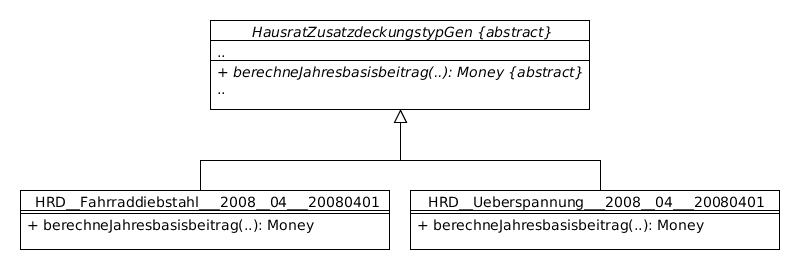
\includegraphics[width=13cm]{./pics/subclassing.png} \caption{Für jeden
Produktbaustein wird eine Subclass angelegt, in der die übersetzte Formel
implementiert ist}
\label{subclassing}
\end{figure}

! verweis auf Tutorial Teil 2

Werden nun die Produktdaten durch einen separaten Service abgerufen, müsste nach
diesem Ansatz auch die Implementierung über den Service abgerufen werden. Ändert
sich in einer neuen Version der Produktdaten eine Formel, muss auch die
Implementierung ausgetauscht werden. Der Classloader von Java sieht jedoch keinen
Austausch von Klassen während des Betriebs vor. Da Application Server im JavaEE
Umfeld selbst diverse Anpassungen am Classloader vornehmen ist eine eigene
Anpassung an dieser Stelle nicht möglich.

! EJB speck verbietet das

Eine Herausforderung im separaten Deployment ist es daher, die Formeln nicht wie
bisher in Subklassen zu kompilieren sondern zur Laufzeit zu interpretieren. Die
Produktdaten werden dadurch frei von Programmcode.

\subsection{Abarbeiten von Anfragen}
! besserer titel
\label{requests}

Mit dem Separaten Deployment von Produktdaten soll es möglich sein, ohne
Unterbrechung des Betriebs der Anwendung neue Produktdaten auszuliefern. Im Fall
eines EJB Services wird also der Produktdaten Service per Hot-Deployment
ausgetauscht.

Nehmen wir an, ein Client\footnote{Als Client bezeichnen wir ein Programm, das
Produktdaten abruft - also der Client des Runtime Repositories} möchte
Produktdaten verarbeiten. Dazu muss er im allgemeinen eine Reihe von Anfragen an
das Repository senden: z.B. fordert der Client einen Produktbaustein an, dann die
aktuell gültige Generation und daraufhin alle assoziierten Produktbausteine. Für
den Client ist dabei wichtig, dass er innerhalb seiner Anfrage auf einem
konsistenten Datenstand arbeitet. Werden während solch einer Anfrage die
Produktdaten ausgetatuscht, muss der Client entweder weiter mit den alten Daten
versorgt werden oder muss eine Exception erhalten und seinen Request abbrechen.

Um bei einem neuen Versuch mit den neuen Daten weiter zu arbeiten, muss der
Client den Beginn seiner Anfrage signalisieren. Das Runtime Repository kann
daraufhin die neuen Produktdaten laden und an den Client weiterleiten. Dabei ist
darauf zu achten, dass ein anderer Client, der sich noch in einer Anfrage
befindet, immernoch eine Exception auslösen muss.

\section{Lösungen}

\subsection{Überblick der Architektur}

Um die im folgenden vorgestellte Lösung zu verwenden, werden
die Runtime Addons\footnote{Dateiname des Archivs:
faktorips-runtime-addons-[version].zip} von Faktor-IPS beötigt. Das Archiv kann
über die Download-Site\footnote{http://update.faktorzehn.org/faktorips/cgi/download.pl?subfolder=v3} heruntergeladen werden.

Wie bereits in der Einleitung erwähnt, betrachten wir die Auslieferung in einem
Java EE Umfeld. Die verschiedenen Programmteile werden als Services implementiert
und in einem EAR ausgeliefert.

Wie bisher wird der Programmcode mit den Modellklassen in einem Archiv gekapselt.
Anstatt des $ClassloaderRuntimeRepositorie$s wird eine neue Implementierung des
Interfaces $IRuntimeRepository$ verwendet: das
$DerivedContentRuntimeRepository$. Dieses ruft zum Laden der Produktdaten einen separaten Service auf, den
Product-Data-Service. Im Klassenpfad des Product-Data-Service sind die
Produktdaten weiterhin als XML-Ressourcen enthalten und können vom Service als
Ressourcen geladen werden.

\begin{figure}[htb] \centering
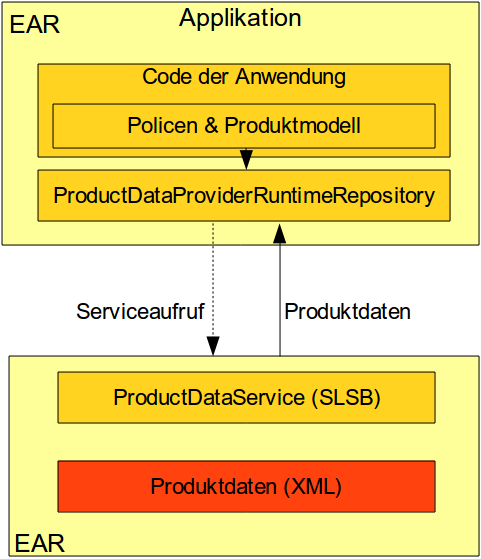
\includegraphics[width=8cm]{./pics/service_architecture.png} \caption{Die
Produktdaten werden in einem separaten Service ausgeliefert der vom Runtime
Repository verwendet wird}
\label{service_architecture}
\end{figure}

Der Product-Data-Service wird als Stateless Session Bean (SLSB) implementiert.
Die Produktdaten werden als XML-Ressourcen geladen, der Inhalt wird an das
Runtime Repository übergeben. Die Instantiierung findet weiterhin im Runtime
Repository statt.

\subsection{Interpretation von Formeln}

! gegenwart: ... gibt es jetzt folgenden

Um die Formeln nicht in Subklassen zu implementieren muss ein Mechanismus zum
Interpretieren des Formel-Codes geschaffen werden. Da das Compilieren der Formeln
in Java-Code bereits existiert, ist die die naheliegenste Lösung diesen
Mechanismus weiter zu verwenden. Der Java-Code wird dazu in das XML der
Produktbausteine geschrieben. Zur Laufzeit wird der Code von
Groovy\footnote{http://groovy.codehaus.org/} ausgeführt. Die Produktdaten
enthalten dadurch keinen Programmcode und sind unabhängig vom Classloader der
Applikation.

\subsection{Abarbeiten von Anfragen}

Um innerhalb einer Anfrage einen konsistenten Datenstand zu gewährleisten, ist es
notwendig, dass ein Client den Beginn seiner Anfrage ankündigt. Nach dem
optimistischen Locking Verfahren kann die Anfrage abgearbeitet werden, bis es zu
einem Fehler kommt. Wenn ein Fehler auftritt muss die Anfrage neu gestartet
werden. Da der Austausch von Produktdaten nicht besonders oft auftritt, ist
dieses Locking Verhalten völlig ausreichend.

Um dieses Locking zu realisieren wird ein Runtime Repository Manager eingeführt.
Jeder Client erhält zunächst anstatt des Runtime Reposiories einen Manager.
Möchte ein Client eine neue Anfrage starteten, ruft er die Methode
$getActualRuntimeRepository()$ am Manager auf. Der Manager liefert daraufhin ein
Runtime Repository mit dem der Client auf den aktuell gültigen Produktdaten
arbeiten kann. Vor der nächsten Anfrage holt sich der Client erneut das aktuelle
Repository. Haben sich die Produktdaten nicht geändert, wird das gleiche
Repository zurück gegeben. Dieser Ablauf ist im Sequenzdiagramm in
Abbildung \ref{clientSequenceEasy} abgebildet.

\begin{figure}[htb] \centering
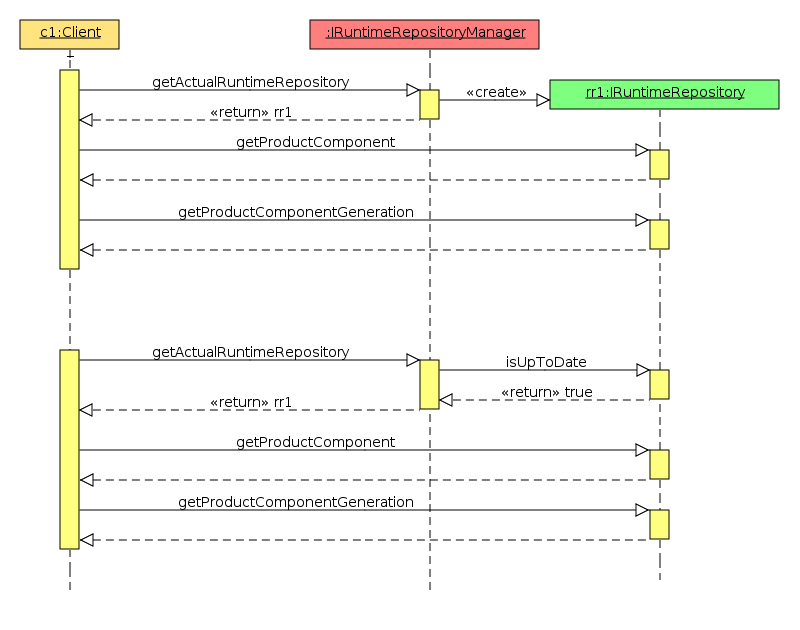
\includegraphics[width=13cm]{./pics/clientSequenceEasy.png} \caption{Der Client
holt sich vor Beginn einer Anfrage das aktuelle Runtime Repository; solange sich
keine Daten ändern arbeitet er auf dem gleichen Repository weiter.}
\label{clientSequenceEasy}
\end{figure}

Werden während der Anfrage die Produktdaten ausgetauscht wirft das Runtime
Repository beim nächsten Abruf von
Produktdaten eine $DataModifiedRuntimeException$. Der Client muss
daraufhin seine Anfrage abbrechen.

Um eine neue Anfrage mit geänderten Produktdaten zu starten wird vom Manager ein
neues Repository geholt. Der Manager stellt die geänderten Produktdaten
fest und erzezgt ein neues Runtime Repository. Der Client arbeitet nun auf
den neuen Produktdaten. Dieses Verhalten ist
im Sequenzdiagramm in Abbildung \ref{clientSequenceChange} dargestellt.

\begin{figure}[htb] \centering
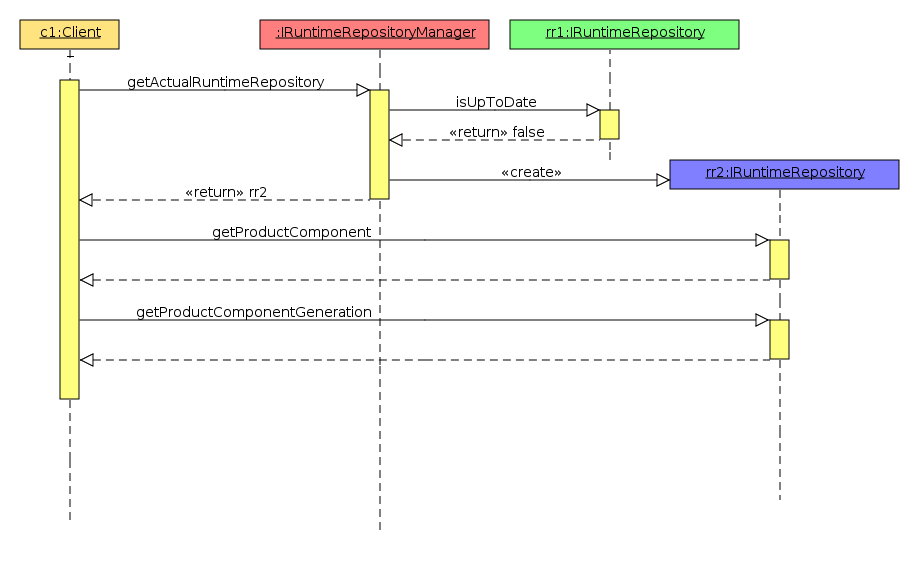
\includegraphics[width=\textwidth]{./pics/clientSequenceChange.png} \caption{Der
Manager stellt fest, dass sich die Produktdaten geändert haben und erstellt ein
neues Runtime Repository}
\label{clientSequenceChange}
\end{figure}

Um die Performance der Abfragen zu erhöhen, enthalten Runtime Repositories einen
Cache und speichern darin bereits abgefragte Produktdaten. Um die Zahl der
Abbrüche beim Austausch von Produktdaten weiter zu verringern wurde das Runtime
Repository so entwickelt, dass es nur beim Abruf von nicht gespeicherten
Produktdaten einen Fehler wirft - solange der Client nur auf Produktdaten im
Cache zugreift, kann er dadurch seine Anfrage zu ende führen.

Auch der gleichzeitige Zugriff mehrerer Client ist mit dieser Lösung kein
Problem. Lediglich der Abruf des aktuellen Runtime Repositories und der gemeinsam
genutzte Cache müssen Threadsicher implementiert werden.

In der Client-Implementierung ist es sinnvoll, einen Manager an zentraler Stelle
zu konfigurieren, damit alle Clients auf den gleichen Manager zugreifen. Zur
Instantiierung des $DetachedContentRuntimeRepositoryManager$ wird ein
Builder\footnote{Dieser Builder ist nach Item 2 im Buch "`Effective Java"' von
Joshua Bloch \cite{effectiveJava} erstellt und weicht vom bekannten Builder
Design Pattern ab.} verwendet. Der Builder ist als innere Klasse des
Repositories realisiert und erwartet eine Implementierung von $IProductDataProviderFactory$ zum instantiieren des Product-Data-Providers. Optional kann man im Builder weitere Voreinstellungen treffen.
Insbesondere eine Implementierung von $IFormulaEvaluatorFactory$\footnote{z.B.
GroovyFormulaEvaluatorFactory zur Ausführen der Formeln mit Groovy (in den
Addons enthalten)} zum ausführen der Formeln sollte gesetzt werden. Ist der
Builder fertig konfiguriert, wird die Methode $build()$ aufgerufen - als Ergebnis erhält man einen $DetachedContentRuntimeRepositoryManager$. Ein
Beispiel zur Instantiierung des Managers ist in Listing \ref{initManager}
gegeben.

\begin{lstlisting}[caption=Initialize DetachedContentRuntimeRepositoryManager,
label=initManager]
repositoryManager = new DetachedContentRuntimeRepositoryManager
	.Builder(pdpFactory)
	.setFormulaEvaluatorFactory(new GroovyFormulaEvaluatorFactory())
	.build();
\end{lstlisting}

\subsubsection{Verknüpfen mehrerer Repositories}

In den meisten Fällen werden Modell- und Produktdaten in mehrere Projekte
untergliedert. Für den Zugriff auf die Daten muss zur Laufzeit für jedes dieser
Projekte ein eigenes Runtime Repository instantiiert werden. Um direkt mit einer
Abfrage an alle relevanten Daten zu gelangen gibt es die Möglichkeit Runtime
Repositories zu verbinden. Die Implementierung des Runtime Repositories
durchsucht automatisch alle verbundenen Repositories um die gewünschten Daten zu
finden.

Mit der Einführung des Runtime Repository Managers ist es nun Aufgabe des
Managers die Repositories zu erstellen. Es muss damit ebenfalls sichergestellt
werden, dass in einem neuen Repository alle notwendigen Verknüpfungen gesetzt
sind. Da sich auch in verknüpften Repositories Produktdaten ändern können, muss
der Manager außerdem überprüfen, ob sich in einem referenzierten Repository die
Daten geändert haben.

Um diese Aufgaben zu bewältigen werden die Manager analog zu den Runtime
Repositories miteinander verknüpft. Ein Manager kann dadurch alle verbundenen
Manager nach dem aktuellen Repository fragen und entsprechend das eigene
Repository zusammen bauen.

\subsection{Konfiguration des EJB Product-Data-Providers}

Der EJB Product-Data-Provider wird mit den Runtime-Addons von Faktor-IPS zur Verfügung gestellt und
kann von der Faktor-IPS Downloadsite\footnote{http://update.faktorzehn.org/faktorips/cgi/download.pl?subfolder=v3} heruntergeladen werden.

Der Product-Data-Provider muss zusammen mit den Produktdaten als eigenes EAR (oder WAR) gebündelt werden.
Dazu werden folgende Bibliotheken benötigt:
\begin{itemize}
	\item faktorips-runtime.productdataservice.jar
	\item faktorips-runtime.productdataservice.common.jar
\end{itemize}

Um auf den Service zuzugreifen müssen auf der Seite des Runtime Repositories
folgende Bibliotheken eingebunden werden:

\begin{itemize}
	\item faktorips-runtime.productdataprovider.ejbclient
	\item faktorips-runtime.productdataservice.common.jar
\end{itemize}

Der Product-Data-Provider wird über die $ejb-jar.xml$\footnote{Die EJB-Konfiguration liegt im Ordner META-INF} konfiguriert. Das Beispiel in Listing \ref{ejb-jar.xml}
konfiguriert einen Produktdatenservice mit dem EJB-Namen $ProductDataService$. Das TOC-File wird über den Classpath geladen und muss daher im Bundle
vorliegen; der Pfad wird per Injection in die Variable $tocFileName$ gesetzt.

\begin{lstlisting}[caption=Beispiel einer ejb-jar.xml, label=ejb-jar.xml,language=XML]{ejb-jar.xml}
<ejb-jar>
	<enterprise-beans>
		<session>
			<ejb-name>
				ProductDataService
			</ejb-name>
			<business-remote>
				org.faktorips.productdataservice.IProductDataService
			</business-remote>
			<ejb-class>
				org.faktorips.productdataservice.ProductDataService
			</ejb-class>
			<session-type>
				Stateless
			</session-type>
			<env-entry>
				<env-entry-name>
					tocFileName
				</env-entry-name>
				<env-entry-type>
					java.lang.String
				</env-entry-type>
				<env-entry-value>
					org/faktorips/model/faktorips-repository-toc.xml
				</env-entry-value>
				<injection-target>
					<injection-target-class>
						org.faktorips.productdataservice.ProductDataService
					</injection-target-class>
					<injection-target-name>
						tocFileName
					</injection-target-name>
				</injection-target>
			</env-entry>
		</session>
	</enterprise-beans>
</ejb-jar>
\end{lstlisting}

\subsection{Implementierung eigener Product-Data-Providers}

!Gegenwart

Ziel des Separaten Deployments von Produktdaten war es, die Produktdaten
unabhängig von der Applikation ausliefern zu können. Dabei soll es nicht nur
möglich sein, die Daten von einem Service abzurufen. Auch die Abfrage einer
Datenbank sollte mit möglichst geringem Aufwand ermöglicht werden. Dazu wurde die
eigentliche Abrage der Daten unabhängig vom $DerivedContentRuntimeRepository$
implementiert. Dieses ruft über das Interface $IProductDataProvider$ die
Methoden zur Abfrage der Produktdaten auf. Zur Instantiierung des konkreten
Product-Data-Providers erhällt das Runtime Repository eine
$ProductDataProviderFactory$.

Das Interface $IProductDataProvider$ enthält Methoden um die unterschiedlichen
Produktdaten (ProductComponent, TableContent, EnumValue, \ldots) abzufragen.
Außerdem kann das Repository die aktuelle Table-Of-Content laden und die Version
der Produktdaten abfragen.

Um festzustellen, ob zwei Versionen kompatibel sind, wird in der Abstrakten
Implementierung $AbstractProductDataProvider$ ein $IVersionChecker$ verwendet.
Die Überprüfung der Kompatibilität wird dadurch ausgelagert und kann je nach
Umfeld verändert werden. Denkbar wäre beispielsweise, dass zwei Versionen
kompatibel sind, wenn Major- und Minor-Version gleich sind, jedoch die
Micro-Version abweicht.

Zusammenfassend müssen zur Implementierung eigener Product-Data-Providers
folgende Implementierungen erstellt werden:

\begin{itemize}
	\item $IProductDataProvider$ zur Abfrage der Daten und der Version - optional
	kann die Abstrakte Klasse $AbstractProductDataProvider$ verwendet werden
	\item $IProductDataProviderFactory$ zum Erstellen des eigenen
	Product-Data-Providers
	\item Optional eine eigene Implementierung von $IVersionChecker$
\end{itemize}


\bibliography{literatur}

\end{document}
